\documentclass[12pt]{article}

\usepackage{graphicx}
\usepackage{sidecap}
\usepackage{geometry}
 \geometry{
 a4paper,
 total={170mm,257mm},
 left=10mm,
 right=10mm,
 top=10mm,
 bottom=10mm
 }
\begin{document}
\begin{titlepage}
   \vspace*{\stretch{1.0}}
   \begin{center}
      \Large\textbf{Weekly Report}\\
      \large\textit{Lingzhen Chen}
   \end{center}
   \vspace*{\stretch{2.0}}
\end{titlepage}

Before we train the vectors on recipe files, some pre-precessing on the data is done. The recipes with less than 3 ingredients are deleted from the training file (the recipe file). And while training, the parameter $min-count$ (minimum occurrence of the ingredient in training file ) is set to 75, which makes the number of valid ingredient 248 out of 381. However it still covers 52375 recipes (more than 95\% percent of the original recipe file)

The recipe vector $I_R$ is represented in one-hot encoding with shape (248,). 

As suggested, we measure the similarity of ingredients by the similarity of their context, i.e. the recipes they are in. For example, we have ingredient $i$ and ingredient $j$, the sets of recipes contains them are represented by $I$ and $J$. Hence the similarity between ingredient $i$ and ingredient $j$ is given by:

\begin{equation}
sim(i,j) = \frac{2 \cdot \sum_{I_{R_i} \in I} \sum_{ I_{R_j} \in J} |I_{R_i} \cap I_{R_j}|}{\sum_{I_{R_i} \in I} |I_{R_i}| + \sum_{I_{R_j} \in J} |I_{R_j}|}
\end{equation}

Intuitively, it is summing up the value of pair-wise dot product of the recipe that contains ingredient $i$ and the recipe that contains ingredient $j$ between all the pairs in $I$ and $J$. Then this value is divided by the scalar product of numbers of elements in $I$ and $J$ (i.e. the number of recipes contains ingredient $i$ multiply that contains ingredient $j$).

By plotting the pair-wise similarity distribution, we have graph as below:

\begin{center}
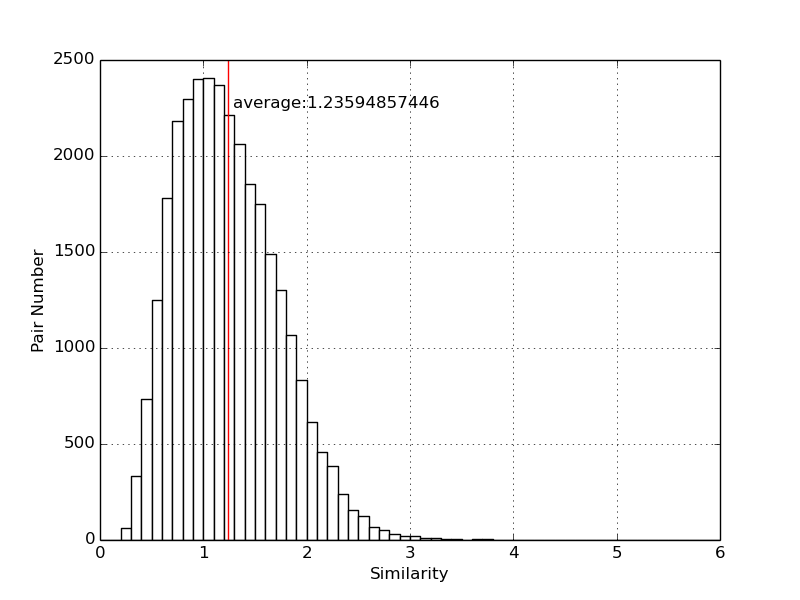
\includegraphics[width=6in]{similarity_distribution.png}
\end{center}

The maximum similarity is 5.5934 whereas the minimum is 0.2091, and among 30628 possible ingredient pairs only 2238 pairs has similarity higher than 2.0. For all the ingredients, the average similarity is given by
\begin{equation}
avg\_similarity = \frac{2}{n(n-1)}\sum_{i=0}^{N}\sum_{j=i+1}^{N}sim(i,j)
\end{equation}
where $N$=248.
By running the scripts, we obtain $avg\_similarity=1.2359$.
Now if we calculate the similarities inside each food category, we obtain result as below:

\begin{center}
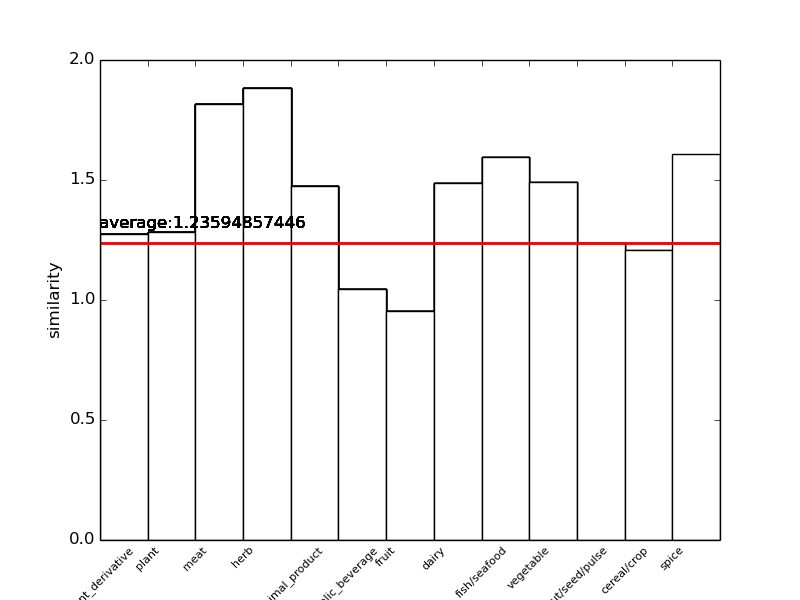
\includegraphics[width=6in]{similarity_by_category.png}
\end{center}

As we can see, not all the food categories has its average similarity of ingredients higher than the average. This could be because ingredients in these categories, like alcoholic\_beverage, fruit or cereal/crop, they are not used restrictedly in a certain type of recipe. For example, they can appear in first dish, second dish, cocktail, sweet and so on. Hence the context of the ingredient is not as similar as others.

Afterwards, experiments are done with fine-tuning the hyper-parameter of the training model, i.e. the parameters used for training with word2vec. Some critical parameters are $-size, -negative, -window, -cbow, -hs, -sample, and -min-count$.

$-cbow$ is used to define if we are using continues bag of word model (-cbow 1) or skip gram model (-cbow 0); from literature, skip-gram model works better with low frequency words, but eventually these two model should generate similar results

$hs$ if use hierarchical softmax or not

$-size$ defines the dimension of vector that we want to obtain

$-negative$ defines the number of negative samples that we want to use during training

$-window$ defines the window size surrounding a word that we are considering during training. Here we usually set to the maximum of total ingredient number in recipe \-32

$-sample$ mainly affects the speed of training, and do not affect the result much

$-min-count$ the minimum times a word occur that it is considered in the vocabulary

Hence the parameters for tuning come down to $size negative cbow$ and $hs$. The range of parameters for experimenting are:

\begin{table}[h]
\centering
\caption{Hyper-parameter range}
\label{my-label}
\begin{tabular}{|l|l|}
\hline
size     & \{5,10,15,20,...,95,100\}   \\ \hline
negative & \{1,2,3,...,20\}           \\ \hline
cbow     & \{0,1\}        \\ \hline
hs       & \{0,1\}     \\ \hline
\end{tabular}
\end{table}

After we have all the model files from these training setting, hierarchical clustering is used on the vectors and average similarity in each cluster is calculated. Result plotting are shown below:

\begin{center}
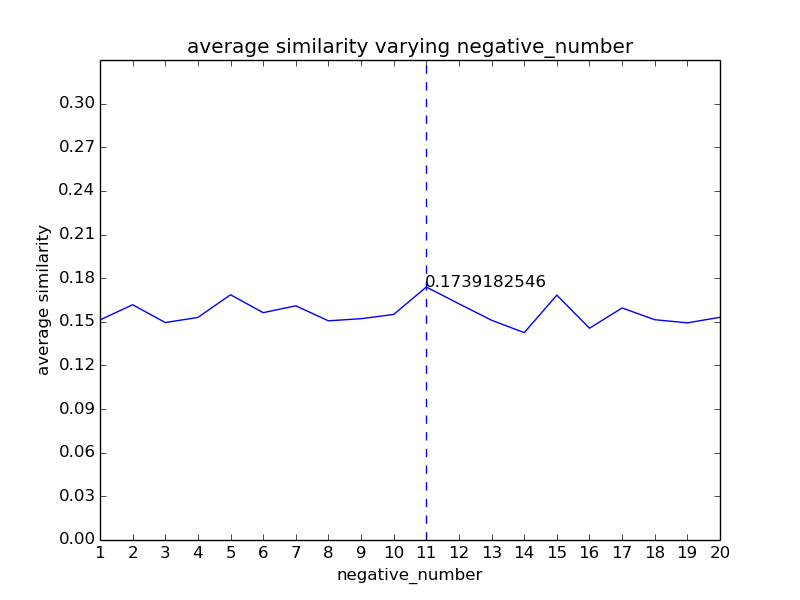
\includegraphics[width=3in]{figure_compare_negative_number.png}
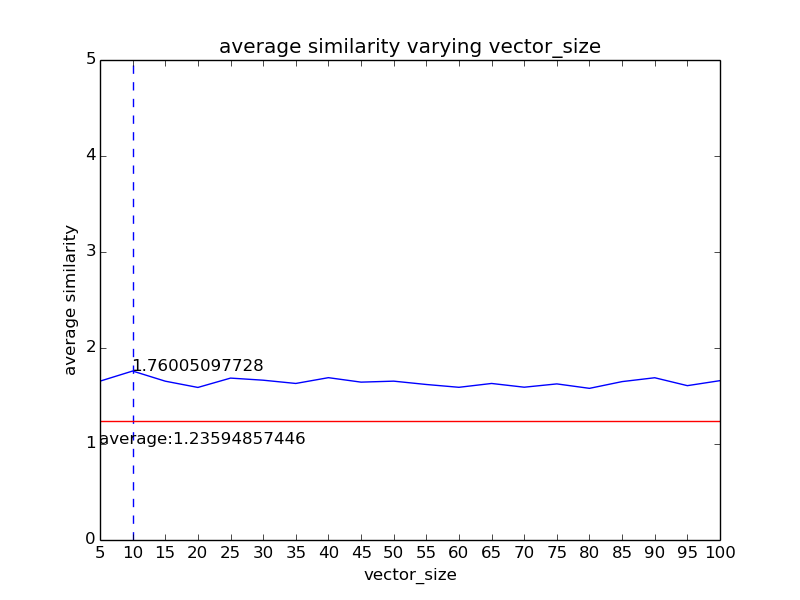
\includegraphics[width=3in]{figure_compare_vector_size.png}
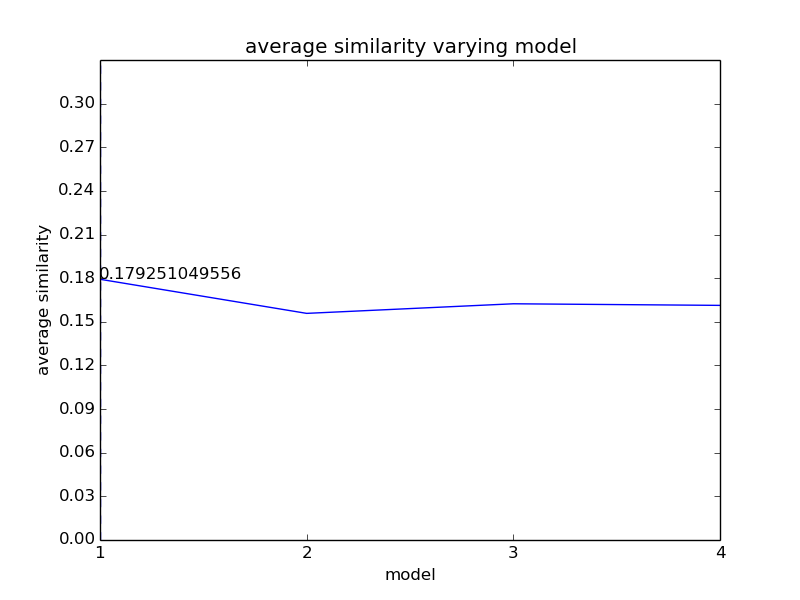
\includegraphics[width=3in]{figure_compare_model.png}
\end{center}

\end{document}
